\chapter{动力系统基础}\label{chap:dynamic}


\section{动力系统概述}
动力系统模型是一种数学工具,用于描述物理系统、生物系统或其他系统随时间演化的行为。它通常基于微分方程或差分方程,通过描述系统内部的状态变量之间的关系来预测系统未来的行为。

动力系统模型可以分为线性模型和非线性模型两种。线性模型假设系统的行为是线性的,通常用线性微分方程或差分方程来描述;而非线性模型则考虑系统的非线性效应,通常需要更复杂的数学形式来描述系统的行为。

在描述动力系统模型时,通常使用微分方程或差分方程的形式来表示动力系统,使用微分方程形式表示的动力系统一般被称为连续动力系统,使用差分方程形式表示的动力系统则被称为离散动力系统。
\begin{defn}[离散动力系统]
    一个离散动力系统可以定义为一个状态空间 $\mathcal{X}$ 上的一组差分方程:
    \begin{equation}\label{eq:discrete_dynamic_system}
        \begin{aligned}
            \mathbf{x}_{n+1} & = \mathbf{f}(\mathbf{x}_n,\mathbf{x_{n-1}},\cdot,\mathbf{x_{x_{n-m}}}), \quad \mathbf{x}_n \in \mathcal{X}, \ n \in \mathbb{N}
        \end{aligned}
    \end{equation}
    其中 $\mathbf{x}_n$ 是状态向量,$\mathbf{f}(\mathbf{x}_n)$ 是系统的动力学方程。这样的动力系统被称为一个$m+1$阶的离散动力系统。
\end{defn}

\begin{defn}[连续动力系统]
    一个连续动力系统可以定义为一个状态空间 $\mathcal{X}$ 上的一组微分方程:
    \begin{equation}\label{eq:dynamic_system}
        \begin{aligned}
            \frac{d\mathbf{x}}{dt} & = \mathbf{f}(\mathbf{x}, t), \quad \mathbf{x} \in \mathcal{X}, \ t \in [0, T]
        \end{aligned}
    \end{equation}
    其中 $\mathbf{x}$ 是状态向量,$\mathbf{f}(\mathbf{x}, t)$ 是系统的动力学方程,$T$ 是观测时间的结束点。
\end{defn}

由于连续动力系统包含的信息往往比离散动力系统多,因此后文中我们主要讨论连续动力系统。

\begin{defn}[混沌]
    在动力系统模型中,如果系统的状态轨迹表现出无规律、无法预测的行为,并且具有灵敏的初始条件依赖性,那么我们称这种状态为混沌。
\end{defn}

当出现混沌时,一个看似简单的确定性系统可能会表现出极不稳定的动力学行为,这种情况下我们很难进行预测,并且微小的误差可能导致结果有很大的不同,因此在使用动力系统模型进行预测时,我们需要特别注意混沌现象的出现。混沌现象的出现同时跟选择的模型以及参数范围有关。

另外,对于动力系统,当$\mathbf{f}$满足一些条件时,对于对应的初值问题有唯一解,有一个定理可以保证这一点。

\begin{thm}[Picard-Lindelöf定理]\label{thm:picard_lindelof}
    对于\ref{eq:dynamic_system}中状态空间为$\mathcal{X}=\mathbb{R}\times\mathbb{R}^n$,设 \( I \) 是一个闭区间,对于初值$(t_0,\mathbf{x_0})\in \textbf{int} I\times\mathbb{R}^n$,其中$\textbf{int} I\times\mathbb{R}^n$表示$I\times\mathbb{R}^n$中的内点,如果 $\mathbf{f}$ 满足对$t$连续,对$\mathbf{x}$Lipschitz连续,则$\exists \epsilon>0$,使得在区间$[t_0-\epsilon,t_0+\epsilon]$上的初值问题有唯一解$\mathbf{x}(t)$。
\end{thm}
\begin{pf}
    让$C_{a,b}=I_a(t_0)\times B_b(\mathbf{x_0})$,其中$I_a(t_0)$是以$t_0$为中心的长度为$a$的区间,$B_b(\mathbf{x_0})$是以$\mathbf{x_0}$为中心的半径为$b$的球。显然$C_{a,b}$是一个紧集,令
    \begin{equation}
        M=\sup_{C_{a,b}}\Vert \mathbf{f}(\mathbf{x},t)\Vert,
    \end{equation}
    并令$L$为$\mathbf{f}$对于$\mathbf{x}$的Lipschitz常数,对于函数空间$\mathcal{C}(I_a(t_0),\mathbf{x_0})$,其中$\mathcal{C}(A,B)$表示所有定义域为$A$,值域为$B$的连续函数,其度量为由无穷范数
    \begin{equation*}
        \Vert\phi\Vert_{\infty}=\sup_{t\in I_a}\Vert\phi(t)\Vert_2。
    \end{equation*}
    诱导的,定义皮卡(Picard)算子:
    \begin{equation*}
        \Gamma:\mathcal{C}(I_a(t_0),\mathbf{x_0})\to \mathcal{C}(I_a(t_0),\mathbf{x_0})\\
        \Gamma(\phi(t))=\mathbf{x_0}+\int_{t_0}^t\mathbf{f}(\phi(s),s)ds
    \end{equation*}
    我们接下来证明这个算子将一个完备度量空间映射到它自己并且是一个压缩映射,对于$\forall \phi\in\mathcal{C}(I_a(t_0),\mathbf{x_0})$,和常函数$c_{\mathbf{x_0}}(I_a)=\mathbf{x_0}$
    \begin{equation*}
        \Vert \Gamma(\phi)-c_{\mathbf{x_0}}\Vert_{\infty}=\Vert\int_{t_0}^t\mathbf{f}(\phi(s),s)ds\Vert_{\infty}\leq \int_{t_0}^{t'}Mds =M|t'-t_0|\leq Ma
    \end{equation*}
    其中$t'$为$\phi(t)$取最大值的点,由于$a$越小,$C_{a,b}$越小,$M$越小,因此取$a^*\leq \frac{b}{M}$,$a=a^*$有
    \begin{equation*}
        \Vert \Gamma(\phi)-c_{\mathbf{x_0}}\Vert_{\infty}\leq b
    \end{equation*}
    即$\Gamma(\phi)\in\mathcal{C}(I_a(t_0),\mathbf{x_0})$,接下来我们只需证$\Gamma$是一个压缩映射。
    \begin{equation*}
        \begin{aligned}
            \Vert\Gamma(\phi_1)-\Gamma(\phi_2)\Vert_{\infty} & =\Vert \int_{t_0}^t\mathbf{f}(\phi_1(s),s)-\mathbf{f}(\phi_2(s),s)ds\Vert_{\infty} \\
                                                             & \leq\int_{t_0}^t\Vert\mathbf{f}(\phi_1(s),s)-\mathbf{f}(\phi_2(s),s)\Vert_2 ds     \\
                                                             & \leq L\int_{t_0}^t\Vert \phi_1(s)-\phi_2(s)\Vert_2 ds                              \\
                                                             & \leq L\int_{t_0}^t\Vert \phi_1-\phi_2\Vert_{\infty} ds                             \\
                                                             & \leq La\Vert \phi_1-\phi_2\Vert_{\infty}
        \end{aligned}
    \end{equation*}
    当$La<1$时,由定义\ref{def:comp_map}可得$\Gamma$为压缩映射,取$a<\frac{1}{L}$,由定理\ref{thm:banach},存在唯一的$\mathbf{x}(t)\in \mathcal{C}(I_a(t_0),\mathbf{x_0})$,$\Gamma(\mathbf{x})=\mathbf{x}$,$\mathbf{x}$为初值问题的唯一解,$a<\min\{\frac{1}{L},\frac{b}{M}\}$
    详细证明可以参考文献\cite{murray2013existence}。
\end{pf}
\begin{rem}\label{rem:P-L}
    对于每个初始条件 $(t_0, \mathbf{x_0})$ 都存在一个唯一的最大(可能无限)开区间
    $$I_{\text{max}} = (t_{-}, t_{+}), \quad t_{\pm} \in \mathbb{R} \cup \{\pm \infty\}, \quad t_0 \in I_{\text{max}}$$
    这样任何满足这个初始条件的解都是满足 $I_{\text{max}}$这个初始条件的解的限制。

    在这种情况下 $t_{\pm} \neq \pm \infty$,只有两种可能:
    \begin{enumerate}
        \item $$\limsup_{t \to t_{\pm}} \|\mathbf{x}(t)\| \to \infty$$
        \item $$\lim_{t \to t_{\pm}} \mathbf{x}(t) \in \partial \bar{\Omega}$$
    \end{enumerate}
    其中 $\Omega$ 是 $\mathbf{f}$ 的定义域,并且 $\partial \bar{\Omega}$ 是它的边界。
\end{rem}
\begin{pf}
    证明思路为\begin{enumerate}
        \item 解的唯一性:假设有两个不同的最大解,那么由Picard-Lindelöf定理可以证明其重叠部分的值相同,将两者不同的部分分别延伸在重叠部分上,则会得到一个更“大”的解(只需验证它满足微分方程),矛盾。因此解唯一
        \item 解的存在性:证明需要用到佐恩引理,构造所有解的并集。
    \end{enumerate}
\end{pf}

\begin{defn}[不动点]
    在动力系统模型中,如果存在一个状态 $\mathbf{x}^*$,使得 $\mathbf{f}(\mathbf{x}^*, t) = 0$,那么我们称这个状态为不动点。
\end{defn}
\begin{defn}[分岔]
    对给定的曲线族,例如矢量场族的积分曲线和微分方程族的解,当其的某个参数发生一些微小改动就会引起整个曲线族拓扑结构发生变化,这些定性的变化称为分岔,发生分岔的参数值称为分岔点。
\end{defn}
对于带参数的动力系统,分岔的研究很重要,其最开始来源于著名数学家庞加莱1885年发表的工作,局部分岔发生在某个分岔点,如果在此处线性化系统得到的雅可比矩阵具有实部为零的特征值则称该分岔为局部分岔,当该特征值等于零时,该分岔是稳定分岔,但如果特征值非零,是纯虚数,则这是Hopf 分岔\cite{enwiki:1216903952}。

在后文模型分析中,我们将会遇到局部分岔的一种:鞍结分岔(saddle-node bifurcation)。
\begin{defn}[鞍结分岔(saddle-node bifurcation)]
    当一个系统中的两个不动点一个鞍点,一个稳定结点随着参数的变化,这两个不动点碰撞并消失,这种现象称为鞍结分岔。两个不动点碰撞对应的点称为鞍结分岔点。
\end{defn}
即便不动点碰撞后消失,它们仍然会对动力系统中的流产生影响,在它们的位置附近会产生一个区域,这个区域会把附近的流吸入并延迟一段时间后流出\cite{strogatz2018nonlinear}。
\section{二维动力系统}
\subsection{二维线性动力系统}
\begin{defn}[二维线性动力系统]

    一个二维线性动力系统可以定义为一个状态空间 $\mathcal{X}$ 上的一组线性微分方程:
    \begin{equation}
        \begin{aligned}
            \dot{x} & = a x + b y, \\
            \dot{y} & = c x + d y,
        \end{aligned}
    \end{equation}
    其中a、b、c、d为参数。
\end{defn}
若用矩阵形式表示,可以令
\begin{equation}
    \mathbf{A}= \begin{pmatrix}
        a & b \\
        c & d
    \end{pmatrix},\mathbf{x}=\begin{pmatrix}
        x \\y
    \end{pmatrix}
\end{equation}
该系统写为
\begin{equation}
    \dot{\mathbf{x}}=\mathbf{A}\mathbf{x}
\end{equation}
由于任意两个解$\mathbf{x_1},\mathbf{x_2}$的线性组合$c_1\mathbf{x_1}+c_2\mathbf{x_2}$也是这个系统的解,因此称这类系统为线性的。注意到当$\mathbf{x^*}=\mathbf{0}$时,$\dot{\mathbf{x}}=\mathbf{0}$,因此$\mathbf{0}$是线性动力系统的一个不动点。
\begin{defn}[闭轨]

    在数学和力学领域,闭轨(closed orbit)是指一个在给定的动力系统中,系统状态在相位空间(phase space)中的一条轨迹,最终又回到起始状态并重复自身。换句话说,闭轨是一条闭合的轨迹,起始点与终点相同。
\end{defn}
闭轨的主要特征包括:
\begin{itemize}
    \item \textbf{周期性}:轨迹是周期性的,即系统的状态在一定时间周期后会回到初始状态。
    \item \textbf{封闭性}:轨迹形成一个闭合的环路,没有开口。
    \item \textbf{稳定性}:在动力系统中,闭轨通常与稳定点、周期轨道或混沌行为相关联。如果一个轨迹在小扰动后依然保持稳定,它可能是一个稳定的闭轨。
\end{itemize}
\subsection{不动点分类}
我们引入一些不动点的稳定性术语
\begin{defn}[全局稳定(Global Stable)]

    一个系统在其所有初始条件下都会收敛到一个稳定的不动点。
\end{defn}
\begin{defn}[李雅普诺夫稳定(Lyapunov Stable)]

    在不动点$\mathbf{x^*}$附近存在一个邻域,对于任意$\epsilon>0$,存在$\delta>0$,使得对于任意初始状态$\mathbf{x_0}$,只要$\Vert \mathbf{x_0}-\mathbf{x^*}\Vert<\delta$,则有$\Vert \mathbf{x_0(t)}-\mathbf{x^*}\Vert<\epsilon$,其中$\mathbf{x_0(t)}$是系统在初始状态$\mathbf{x_0}$下的运动轨迹。
\end{defn}
\begin{defn}[中性稳定(Neutral Stable)]

    一个不动点是李雅普诺夫稳定的,但不是全局稳定的,则称该不动点是中性稳定的。
\end{defn}
\begin{defn}[渐近稳定(Asymptotic Stable)]

    一个不动点既是全局稳定又是李雅普诺夫稳定的,则称该不动点为渐近稳定的。
\end{defn}
\begin{defn}[不稳定(Instability)]

    一个不动点既不是全局稳定也不是李雅普诺夫稳定的,则称该不动点为不稳定的。
\end{defn}

全局稳定系统:$\frac{dx}{dt}=-x,\frac{dy}{dt}=-y$, 不动点在 $(0, 0)$,是吸引子
\begin{figure}[H]
    \centering
    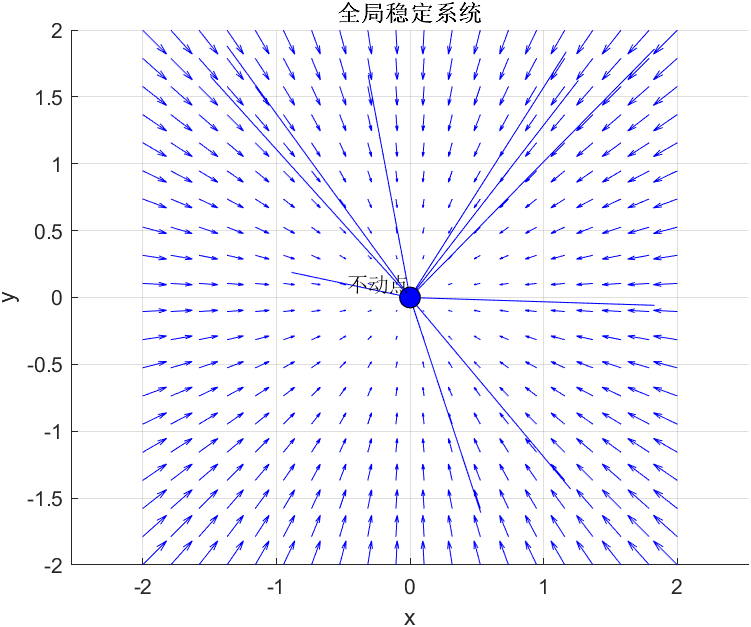
\includegraphics[width=0.8\textwidth]{Img/fix5.png}
    \caption{全局稳定系统}
    \label{fig:global_stable}
\end{figure}
中性稳定系统:$\frac{dx}{dt}=-y,\frac{dy}{dt}=x$, 不动点在 $(0, 0)$,是中性稳定
\begin{figure}[H]
    \centering
    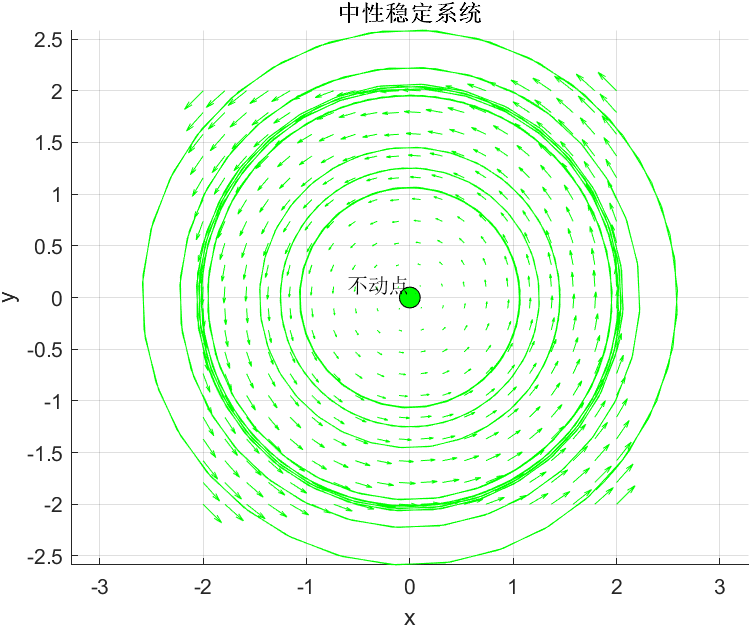
\includegraphics[width=0.8\textwidth]{Img/fix4.png}
    \caption{中性稳定系统}
    \label{fig:neutral_stable}
\end{figure}
不稳定系统:$\frac{dx}{dt}=x-y,\frac{dy}{dt}=x+y$, 不动点在 $(0, 0)$,是排斥子
\begin{figure}[H]
    \centering
    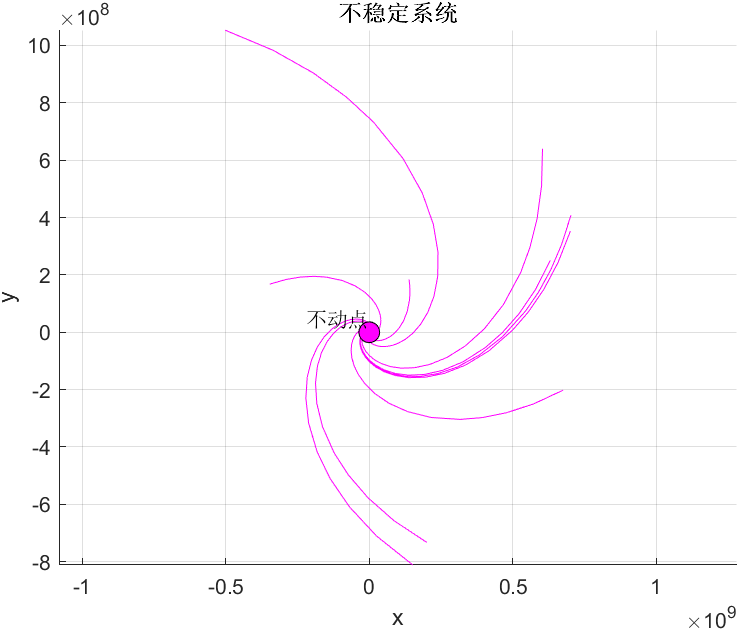
\includegraphics[width=0.8\textwidth]{Img/fix2.png}
    \caption{不稳定系统}
    \label{fig:unstable}
\end{figure}
渐近稳定系统:$\frac{dx}{dt}=-x-y,\frac{dy}{dt}=x-y$, 不动点在 $(0, 0)$,是吸引子
\begin{figure}[H]
    \centering
    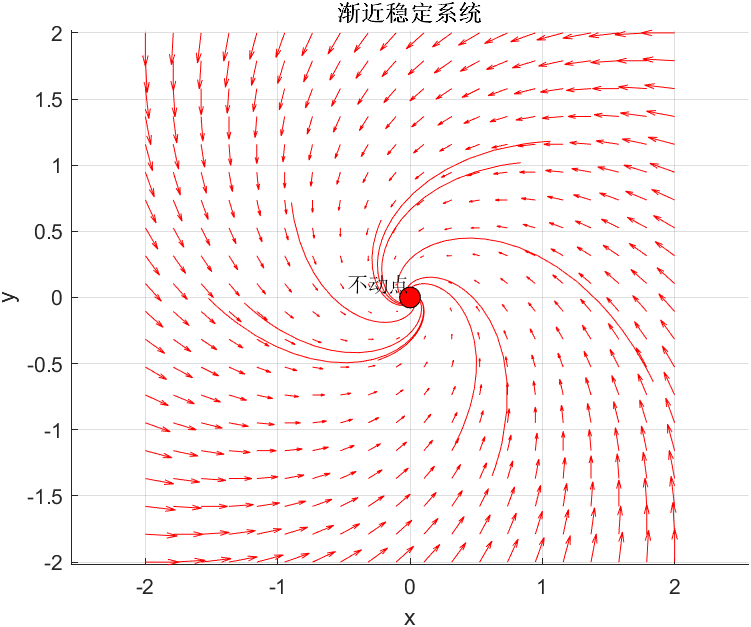
\includegraphics[width=0.8\textwidth]{Img/fix3.png}
    \caption{渐近稳定系统}
    \label{fig:asymptotic_stable}
\end{figure}
一个不动点可以是吸引子,但不是李雅普诺夫稳定的,例如在圆向量场上的:$\frac{d\theta}{dt}=1-\cos\theta$,不动点在$\theta=0$,是吸引子,但不是李雅普诺夫稳定的。
\begin{figure}[H]
    \centering
    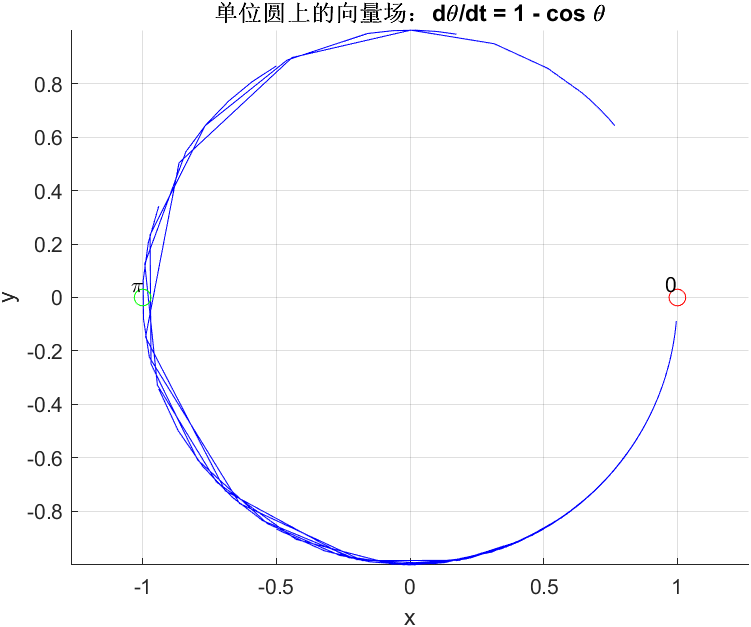
\includegraphics[width=0.8\textwidth]{Img/fix1.png}
    \caption{吸引子但不是李雅普诺夫稳定的系统}
    \label{fig:attractor}
\end{figure}
\subsection{判断不动点分类方法}

对于一个二维线性动力系统,我们可以通过计算矩阵的特征值来判断不动点的稳定性。设$\mathbf{A}$是系统的矩阵,$\lambda_1,\lambda_2$是$\mathbf{A}$的特征值,$\mathbf{v}_1,\mathbf{v}_2$是对应的特征向量。可以发现
\begin{equation}
    \mathbf{x}(t)=c_1e^{\lambda_1t}\mathbf{v}_1+c_2e^{\lambda_2t}\mathbf{v}_2
\end{equation}
因此我们可以发现只要知道了矩阵的特征值就可以判断轨迹的性质。对于二维线性动力系统,我们可以通过计算矩阵的迹和行列式来判断不动点的性质。由定理\ref{thm:trace_det},我们可以得到
\begin{equation}
    \lambda_{1,2}=\frac{1}{2}\left(\text{tr}(\mathbf{A})\pm \sqrt{\text{tr}(\mathbf{A})^2-4\det(\mathbf{A})}\right),\quad \text{tr}(\mathbf{A})=\lambda_1+\lambda_2,\det(\mathbf{A})=\lambda_1\lambda_2
\end{equation}
对于实系数二维线性动力系统,

若$\det(\mathbf{A})<0$,特征值均为实数且符号相反,称不动点为鞍点(saddle)。如图\ref{fig:saddle},鞍点是一个不稳定的不动点,它的一个方向是稳定的,另一个方向是不稳定的。
\begin{figure}[H]
    \centering
    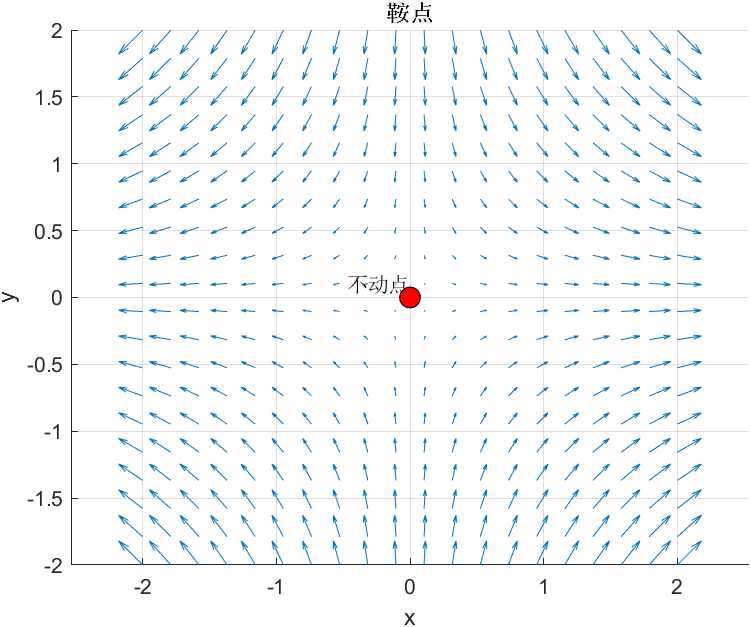
\includegraphics[width=0.8\textwidth]{Img/saddle.png}
    \caption{鞍点}
    \label{fig:saddle}
\end{figure}

如图\ref{fig:node},若$\det(\mathbf{A})>0$,当$\text{tr}(\mathbf{A})^2-4\det(\mathbf{A})>0$时,特征值均为实数且同号,称不动点为结点(node),当$\text{tr}(\mathbf{A})>0$时,称为不稳定结点,当$\text{tr}(\mathbf{A})<0$时,称为稳定结点。当$\text{tr}(\mathbf{A})^2-4\det(\mathbf{A})<0$时,特征值为共轭复数,称不动点为焦点(focus),当$\text{tr}(\mathbf{A})>0$时,称为不稳定焦点,当$\text{tr}(\mathbf{A})<0$时,称为稳定焦点。
\begin{figure}[H]
    \centering
    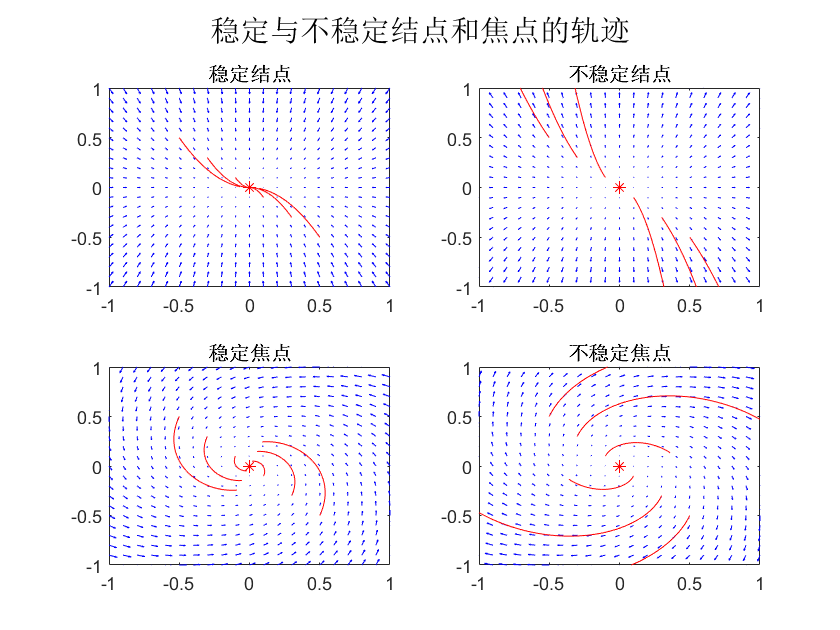
\includegraphics[width=.7\linewidth]{Img/node.png}
    \caption{结点与焦点}
    \label{fig:node}
\end{figure}

如图\ref{fig:star},若$\det(\mathbf{A})>0$,当$\text{tr}(\mathbf{A})=0$时,称不动点为中心(center),中心是一个稳定的不动点。还有一些特殊情况,这些特殊情况都发生在$\text{tr}(\mathbf{A})^2-4\det(\mathbf{A})=0$时,当$\mathbf{A}$特征值相同且有两个线性无关的特征向量时,称不动点为星形结点(star node)。当$\mathbf{A}$特征值相同且只有一个线性无关的特征向量时,称不动点为退化结点(degenerate node)。
\begin{figure}[H]
    \centering
    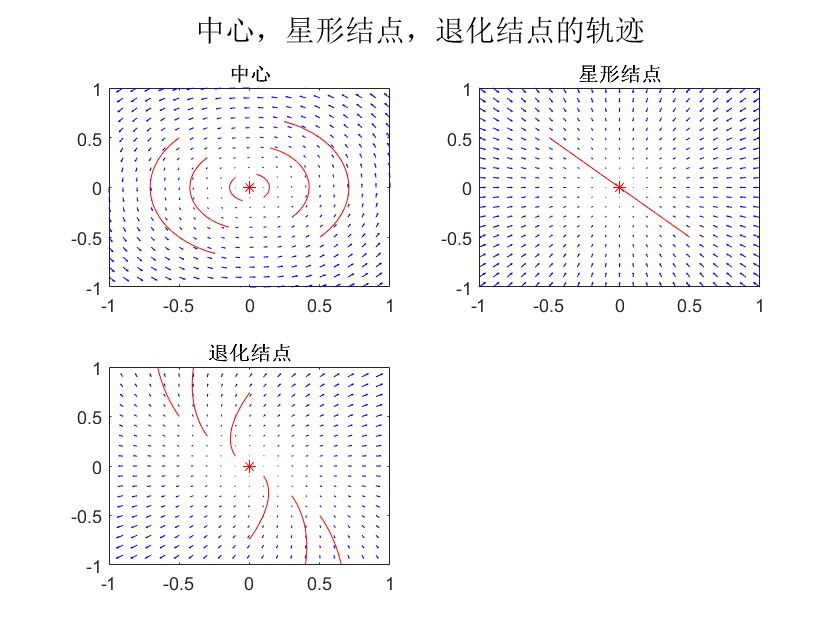
\includegraphics[width=.7\linewidth]{Img/star.png}
    \caption{星形结点与退化结点与中心}
    \label{fig:star}
\end{figure}

若$\det(\mathbf{A})=0$,特征值有一个为零,称不动点为非孤立不动点,此时或者如图\ref{fig:nonisolate},一条直线都是不动点,或者$\mathbf{A}=\mathbf{0}$,一个平面都是不动点。
\begin{figure}[H]
    \centering
    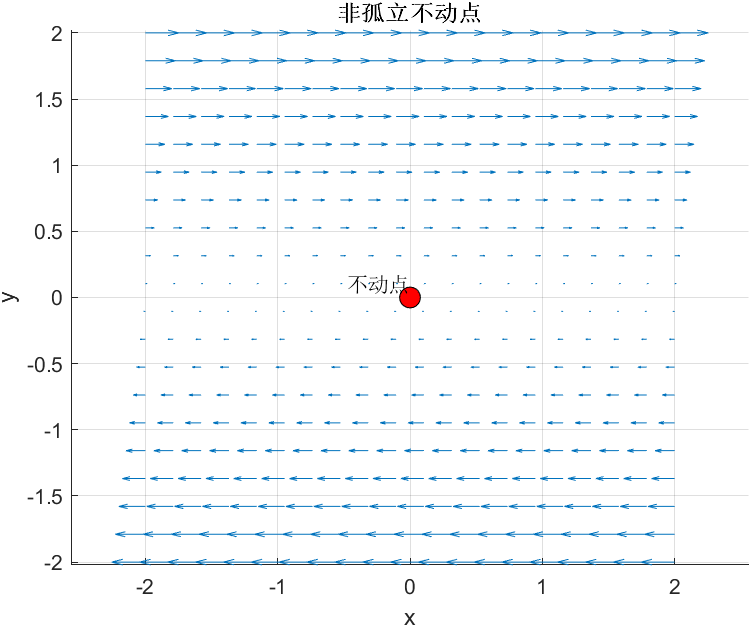
\includegraphics[width=0.8\textwidth]{Img/nonisolate.png}
    \caption{非孤立不动点}
    \label{fig:nonisolate}
\end{figure}
\subsection{二维非线性动力系统}
由于在非线性系统中研究不动点的性质往往比较困难,因此我们通常会考虑一些线性化方法来研究不动点的特性。

考虑系统
\begin{equation}
    \begin{aligned}
        \dot{x}=f(x,y) \\
        \dot{y}=g(x,y)
    \end{aligned}
\end{equation}
假定$(x^*,y^*)$为该系统的一个不动点,通过泰勒展开我们可以得到
\begin{equation}\label{0}
    \begin{pmatrix}
        \dot{u} \\
        \dot{v}
    \end{pmatrix}=
    \begin{pmatrix}
        \frac{\partial f}{\partial x} & \frac{\partial f}{\partial y} \\
        \frac{\partial g}{\partial x} & \frac{\partial g}{\partial y}
    \end{pmatrix}_{(x^*,y^*)}\begin{pmatrix}
        u \\ v
    \end{pmatrix}+\text{二次项}
\end{equation}
其中$(u,v)$为$(x^*,y^*)$处的微小扰动,我们将(\ref{0})中去除二次项的部分称为线性化的系统。
\begin{prop}
    在二维动力系统中,在不动点处线性化的动力系统,只要不动点不在边界处,那么该线性化动力系统的不动点性质与原动力系统相同。
\end{prop}

也就是说如果在线性表达式中可以证明不动点是一个吸引子,那么对于原非线性动力系统,该动力系统也是一个吸引子,具体证明可以参考文献\cite{andronov1974qualitative}。
\begin{defn}[吸引子]
    在动力系统中,如果某一状态或状态集合的邻域内的所有轨迹最终都趋近于该状态或状态集合,则该状态或状态集合称为吸引子。
\end{defn}

\begin{defn}[极限环]
    极限环是一个孤立的闭轨迹, 孤立意味着它附近的轨迹不是闭的,它们盘旋着靠近或原理极限环。如果当时间$t\to +\infty$ 时,所有的邻近轨迹都趋近于极限环,那么所在的流形被称为稳定的,或者称极限环是稳定的(吸引的)。反之,如果$t\to +\infty$ 时,所有的邻近轨迹都远离于极限环,那么称流形是不稳定的或者极限环是不稳定的(非吸引的)。在所有其它情况下,流形既不是稳定也不是不稳定的,或者称极限环是半稳定的。
\end{defn}
\begin{figure}[H]
    \centering
    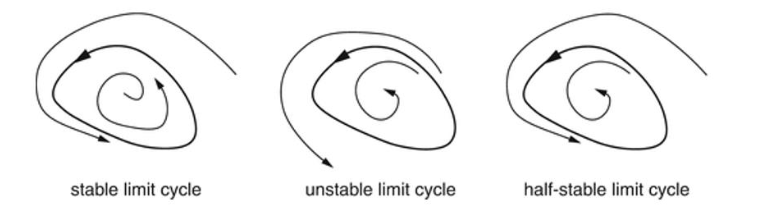
\includegraphics[width=0.8\textwidth]{Img/limit_cycle.png}
    \caption{从左往右依次为稳定极限环,不稳定极限环和半稳定极限环。}
    \label{fig:limit_cycle}
\end{figure}

如图\ref{fig:limit_cycle},极限环分为三种稳定极限环,不稳定极限环和半稳定极限环。稳定极限环是一个吸引子,不稳定极限环是一个排斥子。

稳定极限环模拟了具有自发维持的振荡系统, 如果系统有轻微的扰动,它会自动恢复到标准周期。

\begin{thm}[Dulac准则]
    令$\frac{d\mathbf{x}}{dt}=\mathbf{f}(\mathbf{x})$是一个定义在平面$R$上一个单连通子集的一个连续可微向量场。如果存在一个定义在相应区域上的实值连续可微函数$g(x, y)$,使得$\nabla \cdot (g \frac{d\mathbf{x}}{dt})$不变号,那么$R$上无闭轨。
\end{thm}
\begin{pf}
    假设有一个闭轨$C$在$R$内,令$A$表示$C$内部的区域,由格林公式可得
    \begin{equation}
        \iint_A \nabla \cdot(g \frac{d\mathbf{x}}{dt})dA=\oint_C g \frac{d\mathbf{x}}{dt}\cdot \mathbf{n}dl
    \end{equation}
    显然左边不等于0, 而右边等于0,这与假设矛盾,所以$R$上无闭轨。
\end{pf}

\subsection{庞加莱-本迪克松定理}

考虑二维动力系统
\begin{equation}\label{eq:2d_system}
    \frac{d\mathbf{x}}{dt}=\mathbf{f}(\mathbf{x})
\end{equation}
$\mathbf{f}$是Lipschitz连续的。
\begin{defn}[流]
    对于初值$(0,\mathbf{x_0})$,由\ref{rem:P-L},令$\mathbf{x}(t)$是方程(\ref{eq:2d_system})的唯一最大解,称$\Phi_t(\mathbf{x_0})=\mathbf{x}(t)$为流。
\end{defn}
\begin{rem}
    由定理\ref{thm:picard_lindelof},对$\forall \mathbf{x_0}$,存在$\epsilon>0$满足$\Phi_t(\mathbf{x_0})$在$t\in (-\epsilon,\epsilon)$上是良定义的,事实上$\Phi_t:\mathbb{R}^2\to\mathbb{R}^2$在$\Phi_t$可定义时是Lipschitz连续的。
\end{rem}
\begin{pf}
    由于$\mathbf{f}$是Lipschitz连续的,$\forall \mathbf{x_1},\mathbf{x_2}\in \mathbb{R}^2$,
    \begin{equation}
        \begin{aligned}
            \Vert \mathbf{f}(\mathbf{x_1})-\mathbf{f}(\mathbf{x_2})\Vert & = \Vert \mathbf{x_1}-\mathbf{x_2}+\int_0^t\mathbf{f}(\Phi_s(\mathbf{x_1}))-\mathbf{f}(\Phi_s(\mathbf{x_2}))ds\Vert \\
            &\leq \Vert \mathbf{x_1}-\mathbf{x_2}\Vert+\int_0^t\Vert \mathbf{f}(\Phi_s(\mathbf{x_1}))-\mathbf{f}(\Phi_s(\mathbf{x_2}))\Vert ds\\
            &\leq \Vert \mathbf{x_1}-\mathbf{x_2}\Vert+L\int_0^t\Vert \Phi_s(\mathbf{x_1})-\Phi_s(\mathbf{x_2})\Vert ds
        \end{aligned}
    \end{equation}
    令$u(t)=\Phi_t(\mathbf{x_1})-\Phi_t(\mathbf{x_2})$,$\alpha(t)= \mathbf{x_1}-\mathbf{x_2}$,$\beta(t)=1$,显然$u,\alpha,\beta$满足Grönwall不等式的条件,由\ref{eq:gronwall2}得
    \begin{equation}
        \Vert \Phi_t(\mathbf{x_1})-\Phi_t(\mathbf{x_2})\Vert\leq \Vert \mathbf{x_1}-\mathbf{x_2}\Vert e^{L|t|}
    \end{equation}
    对于固定的$t$,$\Phi_t$是Lipschitz连续的。
\end{pf}
\begin{defn}[$\omega$-极限集]

    对于一个初值$\mathbf{x_0}$满足对所有$t\geq 0$,$\Phi_t(\mathbf{x_0})$都是良定义的,定义$\omega$-极限集$\Omega$为
    \begin{equation}
        \Omega=\{\mathbf{y}\in \mathbb{R}^2|\exists t_n\to +\infty,\Phi_{t_n}(\mathbf{x_0})\to \mathbf{y}\}
    \end{equation}
\end{defn}
\begin{prop}\label{prop:omega_limit_set}

    令$\Omega$是流$\Phi_t$的$\omega$-极限集,那么:
    \begin{enumerate}
        \item $\Omega$是闭集;
        \item 若$\mathbf{x}\in \Omega$,那么$\Phi_t(\mathbf{x})\in \Omega$;
        \item 若$\Omega$是有界的,则它也是是连通的;
    \end{enumerate}
\end{prop}
\begin{pf}

    \begin{enumerate}
        \item 由定义可得,$\Omega$可写为
              \begin{equation*}
                  \Omega=\cap_{r\geq 0}\overline{\{\mathbf{x}(t):t\geq r\}}
              \end{equation*}
              闭集的交集仍为闭集,因此$\Omega$是闭集。
        \item 由于系统\ref{eq:2d_system}不显含变量$t$,我们以$\mathbf{x}(t,t_0,x_0)$表示初值问题$(t_0,\mathbf{x_0})$的解,初值问题
              \begin{equation}\label{eq:initial_problem_1}
                  \begin{aligned}
                      \frac{d\mathbf{x}}{dt} & =\mathbf{f}(\mathbf{x}) \\
                      \mathbf{x}(0)          & =\mathbf{x}(t,t_2,x_0)
                  \end{aligned}
              \end{equation}
              等价于初值问题
              \begin{equation}\label{eq:initial_problem_2}
                  \begin{aligned}
                      \frac{d\mathbf{x}}{dt} & =\mathbf{f}(\mathbf{x}) \\
                      \mathbf{x}(t_2)        & =\mathbf{x}(t,t_2,x_0)
                  \end{aligned}
              \end{equation}
              初值问题\ref{eq:initial_problem_1}上的流为$\Phi_{t_1}(\phi_{t_2}(\mathbf{x_0}))$而初值问题\ref{eq:initial_problem_2}上的流为$\phi_{t_1+t_2}(\mathbf{x_0})$,因此$\Phi_{t_1}(\phi_{t_2}(\mathbf{x_0}))=\phi_{t_1+t_2}(\mathbf{x_0})$,即$\Phi_{t_1}\circ\Phi_{t_2}=\Phi_{t_1+t_2}$。

              对于$\mathbf{x}\in\Omega$,$\exists t_n\to +\infty$,$\lim_{n\to\infty}\Phi_{t_n}(\mathbf{x_0})=\mathbf{x}$,因此
              \begin{equation*}
                  \Phi_t(\mathbf{x})=\Phi_{t}(\lim_{n\to\infty}\Phi_{t_n}(\mathbf{x_0}))=\lim_{n\to\infty}\Phi_{t+t_n}(\mathbf{x_0})=\mathbf{x}\in \Omega。
              \end{equation*}
        \item 由于$\Omega$是闭集,且$\Omega$是有界的,因此$\Omega$是紧集,由第二条性质且$\Phi_t$是连续的知$\Omega$是连通的。
    \end{enumerate}
\end{pf}
\begin{exmp}[$\omega$-极限集]

    \begin{enumerate}
        \item 若$\mathbf{x_0}$是一个不动点,显然其对应的流的$\omega$-极限集为$\mathbf{x_0}$。
        \item 若 $\mathbf{x}$ 是一个平衡点,$\mathbf{x_0}$ 是一个满足 $\lim_{t\to\infty}\Phi_t(\mathbf{x_0}) = \mathbf{x}$ 的初始条件,那么 $\mathbf{x}$ 是 $\Phi_t(\mathbf{x_0})$的$\omega$-极限集。
        \item 若$\Phi_t(\mathbf{x_0})$是一个周期轨道,那么$\Phi_t(\mathbf{x_0})$的$\omega$-极限集是这个周期轨道。
    \end{enumerate}
\end{exmp}
\begin{thm}[庞加莱-本迪克松(Poincaré-Bendixson)定理]

    对于系统\ref{eq:2d_system},如果$\Omega$是一个有界非空的$\omega$-极限集,那么要么$\Omega$中含有至少一个不动点,要么$\Omega$是一个闭轨。
\end{thm}
\subsubsection{横截线(Transversal line)}
\begin{defn}[横截线]
    对于二维动力系统\ref{eq:2d_system},横截线是指一条线段$S=\{\lambda\mathbf{x_0}+(1-\lambda)\mathbf{x_1},0\leq \lambda\leq 1\}$,对于$\forall \mathbf{x}\in S$, $\mathbf{f}(\mathbf{x})$不会消失且不平行于$S$。
\end{defn}
\begin{lem}\label{lem:transversal}
对于一条横截线$S$和$\mathbf{x_0}\in S$,存在一个连续可微函数$r:U\to\mathbb{R}$和一个开集$U$满足$\forall \mathbf{x}\in U$,$\Phi_{r(\mathbf{x})}(\mathbf{x})\in S$。
\end{lem}
\begin{pf}
    令$\mathbb{R}^2$中的坐标形式为$(y,z)$,不妨设$\mathbf{x_0}=(0,0)$,$S$为直线$y=0$的一个子集,对于一个很小的$\epsilon$,我么定义$\psi:B_{\epsilon}(0)\times B_{\epsilon}((0,0))\to \mathbb{R}$为
    \begin{equation}
        \psi(t,\mathbf{x})=\pi\circ\Phi_t(\mathbf{x})
    \end{equation}
    此处$\pi$为投影函数,$\pi(y,z)=y$,由于$\Phi_t$是连续可微的,$\psi$也是连续可微的,显然$\psi(0,0)=0$,且$\frac{\partial \psi}{\partial t}(0,0)=\mathbf{f}(\mathbf{x_0})\neq 0$,因此由隐函数定理,该引理成立。
\end{pf}
\subsubsection{单调性}
\begin{prop}\label{prop:monotonicity}
    设$S$是一条横截线,$\mathbf{x}(t)$是一个解,假设$\mathbf{x}(t_0),\mathbf{x}(t_1),\mathbf{x}(t_2)$是$S$上的三个点,且$t_0<t_1<t_2$,那么$\mathbf{x}(t_1)$在$\mathbf{x}(t_0)$和$\mathbf{x}(t_2)$之间。
\end{prop}
\begin{pf}
    考虑曲线$\Gamma\in\mathbb{R}^2$
    \begin{equation}
        \Gamma=\{\mathbf{x}(t),t\in[t_0,t_1]\}\cup\{\lambda\mathbf{x}(t_0)+(1-\lambda)\mathbf{x}(t_1),0\leq \lambda\leq 1\}
    \end{equation}
    由Jordan曲线定理,$\Gamma$将$\mathbb{R}^2$分为两个区域,$D_1,D_2$,由定义可知$\mathbf{f}(\mathbf{x}(t))$不会消失且不平行于$S$,因此$\mathbf{x}(t)$必会在$t_1$后进入$D_1$或$D_2$,不妨设$\mathbf{x}(t)$在$t_1$后进入$D_1$,对于$t^*>t_1$不存在$\mathbf{x}(t^*)$在$\Gamma$上,因为
    \begin{itemize}
        \item 若$\mathbf{x}(t^*)\in \{\mathbf{x}(t),t\in[t_0,t_1]\}$则其与解的唯一性矛盾
        \item 若$\mathbf{x}(t^*)\in \{\lambda\mathbf{x}(t_0)+(1-\lambda)\mathbf{x}(t_1),0\leq \lambda\leq 1\}$由于$\mathbf{f}$在对应的点上指向$D_1$,矛盾
    \end{itemize}
    因此$\mathbf{x}(t_2)\in \text{int}(D_1)$,即$\mathbf{x}(t_1)$在$\mathbf{x}(t_0)$和$\mathbf{x}(t_2)$之间。
\end{pf}
\begin{prop}\label{prop:at_most_one_point}
    对于系统\ref{eq:2d_system},若$\mathbf{x}(t)$是它的解,$\Omega$是其对应的$\omega$-极限集,$S$是一条横截线,那么$\Omega\cap S$最多有一个点。
\end{prop}
\begin{pf}
    我们是用反证法,假设有不同的两点$\mathbf{x_1},\mathbf{x_2}\in\Omega\cap S$,由引理\ref{lem:transversal},存在两个无交开集$U_1,U_2$满足对应条件,由于$\mathbf{x_1},\mathbf{x_2}\in \Omega$,存在两个序列$\{t_n^1\},\{t_n^2\}$满足$\lim_{n\to\infty}\mathbf{x}(t_n^1)=\mathbf{x_1},
    \lim_{n\to\infty}\mathbf{x}(t_n^2)=\mathbf{x_2}$,不妨设$\mathbf{x}(t_n^1)\in U_1,\mathbf{x}(t_n^2)\in U_2$,因此存在$\mathbf{x}(t_n^{1^*})\to\mathbf{x_1}, \mathbf{x}{t_n^{{2^*}}}\to \mathbf{x_2},n\to\infty$,其中$\mathbf{x}(t_n^{1^*})\in S,\mathbf{x}(t_n^{{2^*}})\in S$,在这些里面我们能找到$t_{1}^{1^*}<t_{n_1}^{{2^*}}<t_{n_2}^{1^*}$,显然$\mathbf{x}(t_1^{1^*})\neq \mathbf{x}(t_{n_2}^{1^*})$,但$\mathbf{x}(t_1^{1^*}),\mathbf{x}(t_{n_1}^{{2^*}}),\mathbf{x}(t_{n_2}^{1^*})$不在$S$上单调,这与命题\ref{prop:monotonicity}矛盾,因此$\Omega\cap S$最多有一个点。
\end{pf}
\subsubsection{庞加莱-本迪克松定理证明}

我们将考虑一个有界的$\omega$-极限集$\Omega$,其中不包含任何不动点,我们将证明这种情况下$\Omega$是一个闭轨。证明将分为两步,第一步证明$\Omega$中的点都是周期的,第二步证明这些点的图像就是$\Omega$。
\begin{prop}\label{prop:periodic_orbit}
    令$\Omega$是解$\Phi_t(\mathbf{x_0})$的$\omega$-极限集,$\Omega$不包含任何不动点,且非空有界,那么对于$\mathbf{y}\in \Omega$,$\Phi_t(\mathbf{y})$是一个周期轨道。
\end{prop}
\begin{pf}
    由命题\ref{prop:omega_limit_set},当$\Phi_t(\mathbf{y})$有定义时,$\Phi_t(\mathbf{y})\in \Omega$,因此$\Phi_t(\mathbf{y})$是周期轨道。由\ref{rem:P-L}$\Phi_t(\mathbf{y})$在$t\geq 0$时都是良定义的,由于$\{\Phi_t(\mathbf{y})\}_{t\geq 0}$是有界的,由Bolzano-Weierstrass定理,存在一个序列$\{t_n\}_{n\to\infty}$和一个点$\mathbf{z}$满足$\lim_{n\to\infty}\Phi_{t_n}(\mathbf{y})=\mathbf{z}$,因此$\mathbf{z}\in \Omega$,由于$\Omega$是闭集,$\mathbf{z}\in \Omega$,因此$\Phi_t(\mathbf{z})=\mathbf{z}$,因此$\mathbf{z}$不是一个不动点,我们可以找到一条经过$\mathbf{z}$的横截线$S$。

    由于$\lim_{n\to\infty}\Phi_{t_n}(\mathbf{y})=\mathbf{z}$,由引理\ref{lem:transversal},存在$\{a_k\}_{k=1}^{\infty}$满足$\lim_{k\to\infty}\Phi_{a_k}(\mathbf{y})=\mathbf{z}$,且$\Phi_{a_k}(\mathbf{y})\in S$,因此$\Phi_{a_k}(\mathbf{y})\in \Omega\cap S$,由\ref{prop:at_most_one_point},$\Phi_{a_k}(\mathbf{y})$都是同一个点,即存在$a_m\neq a_n$使得$\Phi_{a_m}(\mathbf{y})=\Phi_{a_n}(\mathbf{y})$,因此$\Phi_t(\mathbf{y})$是一个周期轨道。
\end{pf}
\begin{prop}\label{prop:closed_orbit}
    令$\Omega$是解$\Phi_t(\mathbf{x_0})$的$\omega$-极限集,$\Omega$不包含任何不动点,且非空有界,对于$\mathbf{y}\in\Omega$,$\Omega\setminus\cup_{t\geq 0}\{\Phi_t(\mathbf{y})\}=\emptyset$。
\end{prop}
\begin{pf}
    由命题\ref{prop:omega_limit_set},$\Omega$是连通的,显然$\cup_{t\geq 0}\{\Phi_t(\mathbf{y})\}$是一个非空闭集,因此我们只需证$\Omega\setminus\cup_{t\geq 0}\{\Phi_t(\mathbf{y})\}$是一个闭集。

    取一串柯西列$\{\mathbf{z_k}\}_{k=1}^{\infty}\in \Omega\setminus\cup_{t\geq 0}\{\Phi_t(\mathbf{y})\}$,假设$\lim_{k\to\infty}\mathbf{z_k}=\mathbf{z}$,我们将证明$\mathbf{z}\in \Omega\setminus\cup_{t\geq 0}\{\Phi_t(\mathbf{y})\}$。

    由于$\Omega$是一个闭集,$\mathbf{z}\in \Omega$,因此$\mathbf{z}$不是一个不动点,我们可以取一条通过$\mathbf{z}$的横截线$S$。对于每个$k\in\mathbb{N}$,由于$\mathbf{z_k}\in\Omega$,存在$\{t_{k,l}\}_{l=1}^{\infty}(lim_{l\to\infty}t_{k,l}=\infty)$使得$\lim_{l\to\infty}\Phi_{t_{k,l}}(\mathbf{x_0})=\mathbf{z_k}$,由引理\ref{lem:transversal},对于足够大的$k$满足$\mathbf{z_k}$在$\mathbf{z}$对应的$U$中,我们能找到$\{\hat{t_{k,l}}\}_{l=1}^{\infty}(lim_{l\to\infty}\hat{t_{k,l}}=\infty)$使得$\lim_{l\to\infty}\Phi_{\hat{t_{k,l}}}(\mathbf{x_0})=\mathbf{z_k}$,且$\Phi_{\hat{t_{k,l}}}(\mathbf{x_0})\in S$,由命题\ref{prop:at_most_one_point},这些都是同一个点,因此$\Phi_{\hat{t_{k,l}}}(\mathbf{x_0})=\mathbf{z}$,即对于对应的$k$,$\mathbf{z_n}=\mathbf{z}(n\geq k)$,因此$\mathbf{z}\in \Omega\setminus\cup_{t\geq 0}\{\Phi_t(\mathbf{y})\}$。

    综上所述,$\Omega\setminus\cup_{t\geq 0}\{\Phi_t(\mathbf{y})\}$是一个闭集。
\end{pf}
结合命题\ref{prop:periodic_orbit}和命题\ref{prop:closed_orbit},我们可以得到庞加莱-本迪克松定理。

关于更多证明细节,可以参考Coddington的工作\cite{coddington1956theory}。庞加莱-本迪克松定理表明,混沌永远不会在相平面中产生\cite{strogatz2018nonlinear}。
